\appendix
\phantomsection
\section*{Appendix}
\addcontentsline{toc}{section}{Appendix}
\addtocontents{toc}{\protect\setcounter{tocdepth}{1}}


\section{Gripper Stall charts}




\subsection{Current-based overstepping}
\label{app:stall-current-overstepping}

This chart shows a case where the current based stall detection did not stop the motor cleanly at the stall point. The current signal crosses the threshold repeatedly, but the signal is noisy and does not give a clear single transition from normal movement to stall. Because the software had to wait for repeated samples above the threshold, the motor could continue moving for too long before the stall was accepted.

This caused overstepping, where the gripper moved further than intended after reaching the mechanical resistance. This was one of the reasons why current based stall detection was not selected as the final method.

\begin{figure}[H]
    \centering
    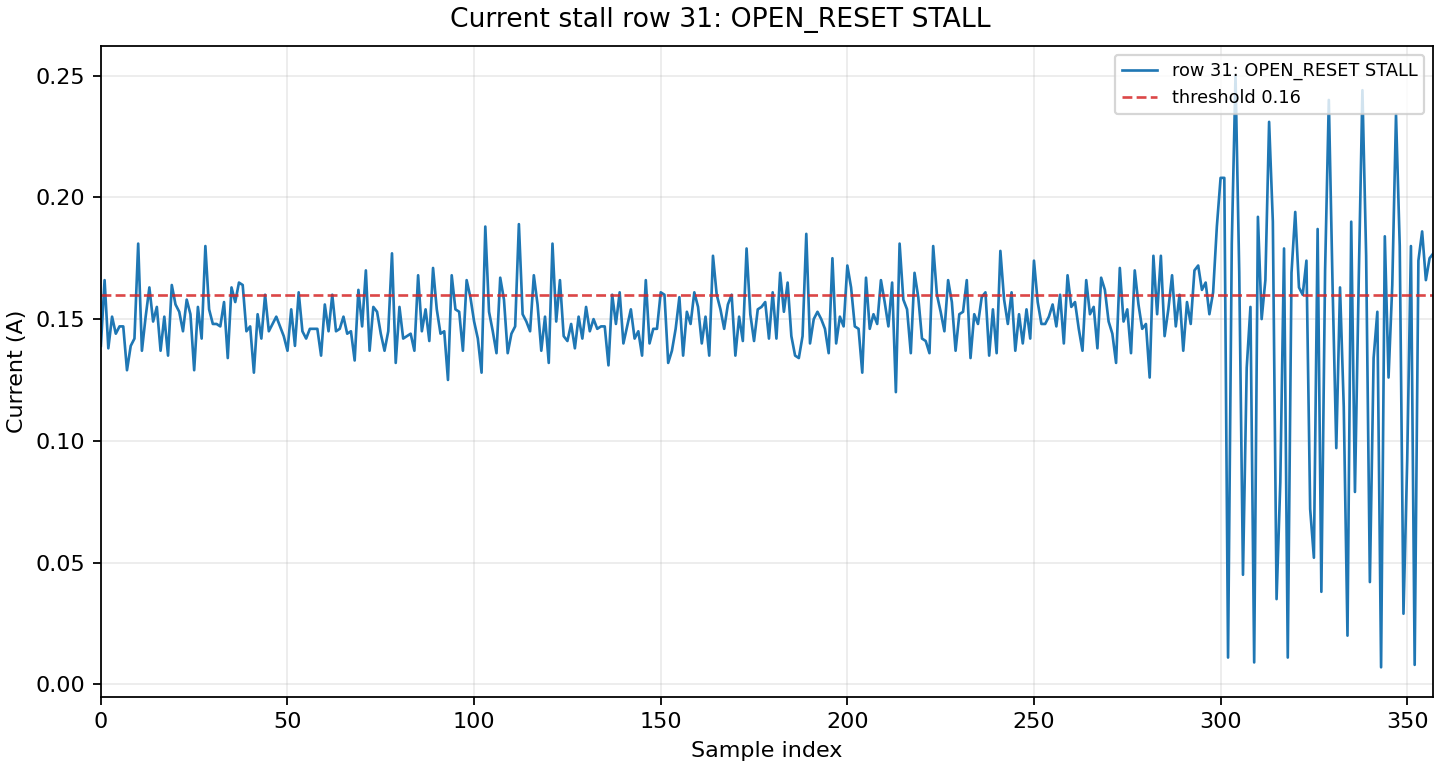
\includegraphics[width=1\textwidth]{Appendix/Images/StallChartOverstepping.png}
    \caption{Current based stall detection with overstepping at stall.}
    \label{fig:stall-chart-with-overstepping}
\end{figure}


\clearpage
\subsection{Stall against hardstop vs. against cube with spring coupling}
\label{app:stall-charts}

The charts show the stall signals recorded during the gripper tests. Both the StallGuard value and the current based stall signal are shown for a hardstop measurement and for gripping an object with the spring coupling extending.

\begin{figure}[H]
    \centering
    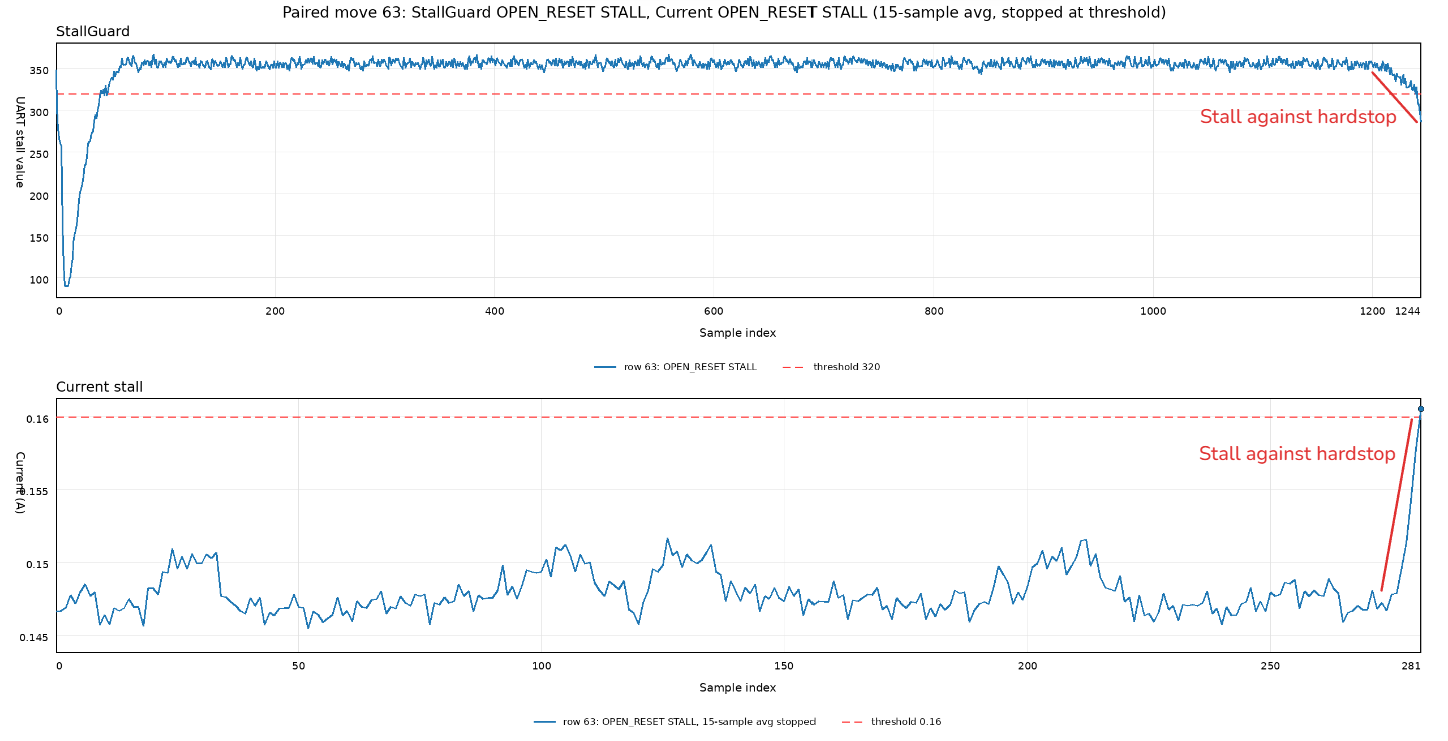
\includegraphics[width=1\textwidth]{Appendix/Images/StallChartHardstop.png}
    \caption{Stall detection measurements when the gripper reaches the hard stop.}
    \label{fig:stall-chart-hard-stop}
\end{figure}

\begin{figure}[H]
    \centering
    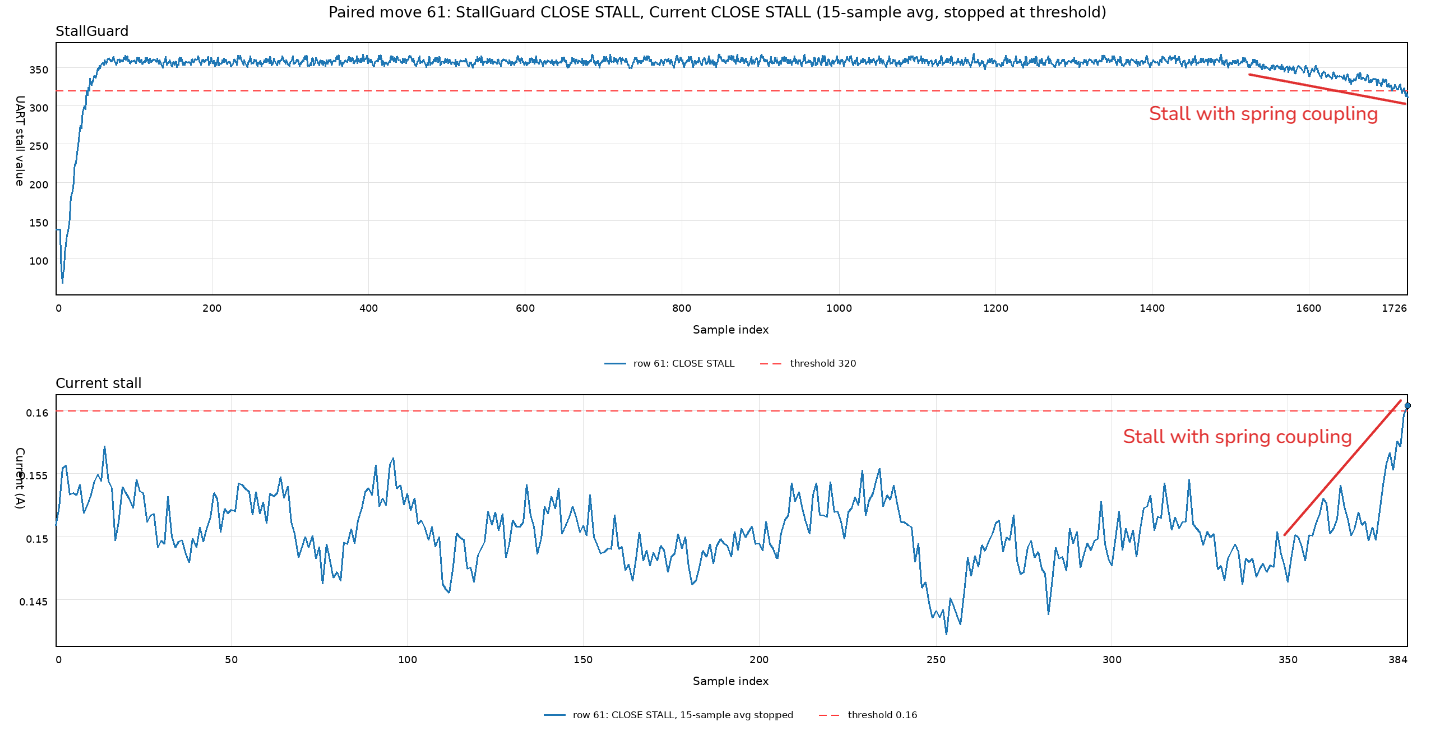
\includegraphics[width=1\textwidth]{Appendix/Images/StallChartWithSpring.png}
    \caption{Stall detection measurements with the spring mechanism.}
    \label{fig:stall-chart-with-spring}
\end{figure}

\clearpage



\section{Storage System Test Data}
\label{app:extra-data-collection}


Default configuration: 100 ms \texttt{sleep\_ms}, read bits synced, read expected.

\begin{table}[H]
\centering
\begin{tabular}{|l|c|c|c|}
\hline
Configuration & Average task time [s] & Irregularity rate & Standard deviation \\
\hline
UR Moving & 3.3 & 10\%& 4\% \\
UR Off & 3.3 & 10\% & 4\% \\

\hline
\end{tabular}
\caption{Encoder performance with and without UR movement to asses the effect of EMI.}
\label{tab:encoder-performance-ur}
\end{table}

Without light the encoder does not work at all! The point is however to determine if extra lighting had a noticeable effect.

Extra lighting also did not improve the result beyond statistical uncertainty  Table \ref{tab:encoder-performance-lighting}. %Appendix~\ref{app:extra-data-collection} 



Default configuration: 0 ms \texttt{sleep\_ms}, read bits synced, read expected.

\begin{table}[H]
\centering
\begin{tabular}{|l|c|c|c|}
\hline
Configuration & Average task time [s] & Irregularity rate & Standard deviation \\
\hline
Default lighting & 3.3 & 13\%& 5\% \\
Extra lighting & 3.3 & 13\% & 6\% \\

\hline
\end{tabular}
\caption{Encoder performance with default and extra lighting.}
\label{tab:encoder-performance-lighting}
\end{table}

The following test was to determine the system reliability at different PWM-levels.

Default configuration: 100 ms \texttt{sleep\_ms}, read bits synced, read expected.

\begin{table}[H]
\centering
\begin{tabular}{|l|c|c|c|}
\hline
Configuration & Average task time [s] & Irregularity rate & Standard deviation \\
\hline
100\% & 3.3 & 13\%& 5\% \\
50\% & 3.6 & 16\% & 7\% \\
5\% & 4.9 & 10\%& 3\% \\

\hline
\end{tabular}
\caption{Encoder performance with different PWM-levels}
\label{tab:encoder-performance-pwm}
\end{table}




\clearpage
\section{Encoder Speed and Timing Calculations}
\label{app:encoder-speed-calculations}

The relative encoder lane was not used in the final implementation because reliable relative encoding would require every transition to be detected while the disk is moving. The following calculations clarify this design choice and display limitations of the LDR based encoder.

The selected LDR has a rise time of approximately 30 ms\cite{gl5528_datasheet}. At the encoder radius of 225 mm to the furthest encoder lane housing the relative encoder lane, the circumference of the encoder path is

\[
C = 2 \pi r = 2 \pi \cdot 225 = 1413.7 \text{ mm}
\]

%Each storage position covers \(45^\circ\), \(360^\circ\) / 8 slots and 

The relative encoder marking width was approximately \(4.5^\circ\). The physical length of one encoder marking is therefore

\[
L = C \cdot \frac{4.5}{360}
\]

\[
L = 1413.7 \cdot \frac{4.5}{360} = 17.7 \text{ mm}
\]

This is the distance that the LDR has to detect at least 2 measurements to be sure of at least one of them recording the engraved section

This gives a maximum travel distance per sample of

\[
s = \frac{17.7}{2} = 8.85 \text{ mm}
\]

Using the LDR rise time of 30 ms \cite{gl5528_datasheet}, the maximum theoretical encoder speed becomes

\[
v = \frac{8.85}{0.030} = 295 \text{ mm/s}
\]

Converted to rotational speed:

\[
n = \frac{v}{C} \cdot 60
\]

\[
n = \frac{295}{1413.7} \cdot 60 = 12.5 \text{ RPM}
\]

This means that, based only on the LDR rise time, the encoder should rotate below approximately 12.5 RPM to reliably detect the relative encoder markings.

%This does not take software lootime, I2C communication delay or averaging of value into consideration.

The motor speed at 100\% PWM was measured to be slightly above 15 RPM, which is close to the datasheet value of 14.5 RPM for the selected geared motor \cite{nidec_hg37_datasheet}. With the 1:3 belt reduction, the disk speed was reduced to approximately

\[
n_\text{disk} = \frac{15}{3} = 5 \text{ RPM}
\]

This suggests that the disk speed should be within the theoretical limit set by the LDR rise time. However, practical testing showed that the LDR rise time was not the main limiting factor.

When only raw LDR values were read, the average interval between readings was approximately 38 ms after subtracting the intentional \texttt{sleep\_ms} delay. Using the same two-sample requirement, this gives a practical speed estimate of

\[
v = \frac{8.85}{0.038} = 232.9 \text{ mm/s}
\]

\[
n = \frac{232.9}{1413.7} \cdot 60 = 9.9 \text{ RPM}
\]

This estimate does not include the additional delay from averaging several ADC samples during normal operation. Therefore, the practical reading speed was lower than the theoretical LDR response time alone suggested.

The calculations show why the absolute encoder was preferred over the relative encoder lane. The absolute encoder does not require every transition to be detected. Instead, each valid encoder reading directly identifies the current storage position. This made the system more tolerant of missed or rejected intermediate readings.
\clearpage

\section{2-hour test results}
\label{app:2HourResults}

\providecommand{\thickhline}{\noalign{\hrule height 1.2pt}}

\begin{center}
  \rotatebox{90}{%
    \resizebox{0.85\textheight}{!}{%
      \centering
      \begin{tabular}{|c|c|c|c|c|c|c|c|}
        \hline
        \textbf{Subsystem} & \textbf{Error type} & \textbf{0-30min} & \textbf{30-60min} & \textbf{60-90min} & \textbf{90-120min} & \textbf{Error type total} & \textbf{Subsystem total} \\
        \thickhline
        \textit{Vision} & Can't read QR & 3 & 2 & 2 & 2 & 9 & 14 \\
        \hline
        & Can't find QR & 0 & 0 & 0 & 0 & 0 &  \\
        \hline
        & Slow to read QR & 1 & 1 & 0 & 3 & 5 &  \\
        \hline
        & Wrong coordinates & 0 & 0 & 0 & 0 & 0 &  \\
        \hline
        &  &  &  &  &  &  &  \\
        %\\
        \thickhline
        \textit{Storage} & Wrong slot & 0 & 0 & 1 & 2 & 3 & 15 \\
        \hline
        & Cannot find slot & 0 & 3 & 3 & 1 & 7 &  \\
        \hline
        & Difficulty finding slot & 0 & 0 & 1 & 0 & 1 &  \\
        \hline
        & Offset buildup & 0 & 0 & 1 & 1 & 2 &  \\
        \hline
        & Cube displacement & 0 & 1 & 0 & 1 & 2 &  \\
        \hline
        &  &  &  &  &  &  &  \\
        %\\
        \thickhline
        \textit{Gripper} & No grip & 0 & 0 & 0 & 0 & 0 & 1 \\
        \hline
        & Other & 0 & 1 & 0 & 0 & 1 &  \\
        \hline
        &  &  &  &  &  &  &  \\
        %\\
        \thickhline
        \textit{Robot} & No movement & 0 & 0 & 0 & 0 & 0 & 0 \\
        \hline
        & Wrong movement & 0 & 0 & 0 & 0 & 0 &  \\
        \hline
        &  &  &  &  &  &  &  \\
        %\\
        \thickhline
        \textit{PC} & Stalling & 1 & 0 & 0 & 0 & 1 & 1 \\
        \hline
        %&  &  &  &  &  &  &  \\
        %\\
        \hline
        \thickhline
        \textbf{Cycles} &  & 20 & 21 & 20 & 20 & 81 & 81 \\
        \hline
      \end{tabular}
    }%
  }
  \captionof{table}{2-hour test results (errors \& cycles)}
  \label{tab:2hour-test-results}
\end{center}
\clearpage

\section{Additional Figures}

\subsection{Test setup of the machine}
\label{app:test-setup}

\begin{figure}[H]
    \centering
    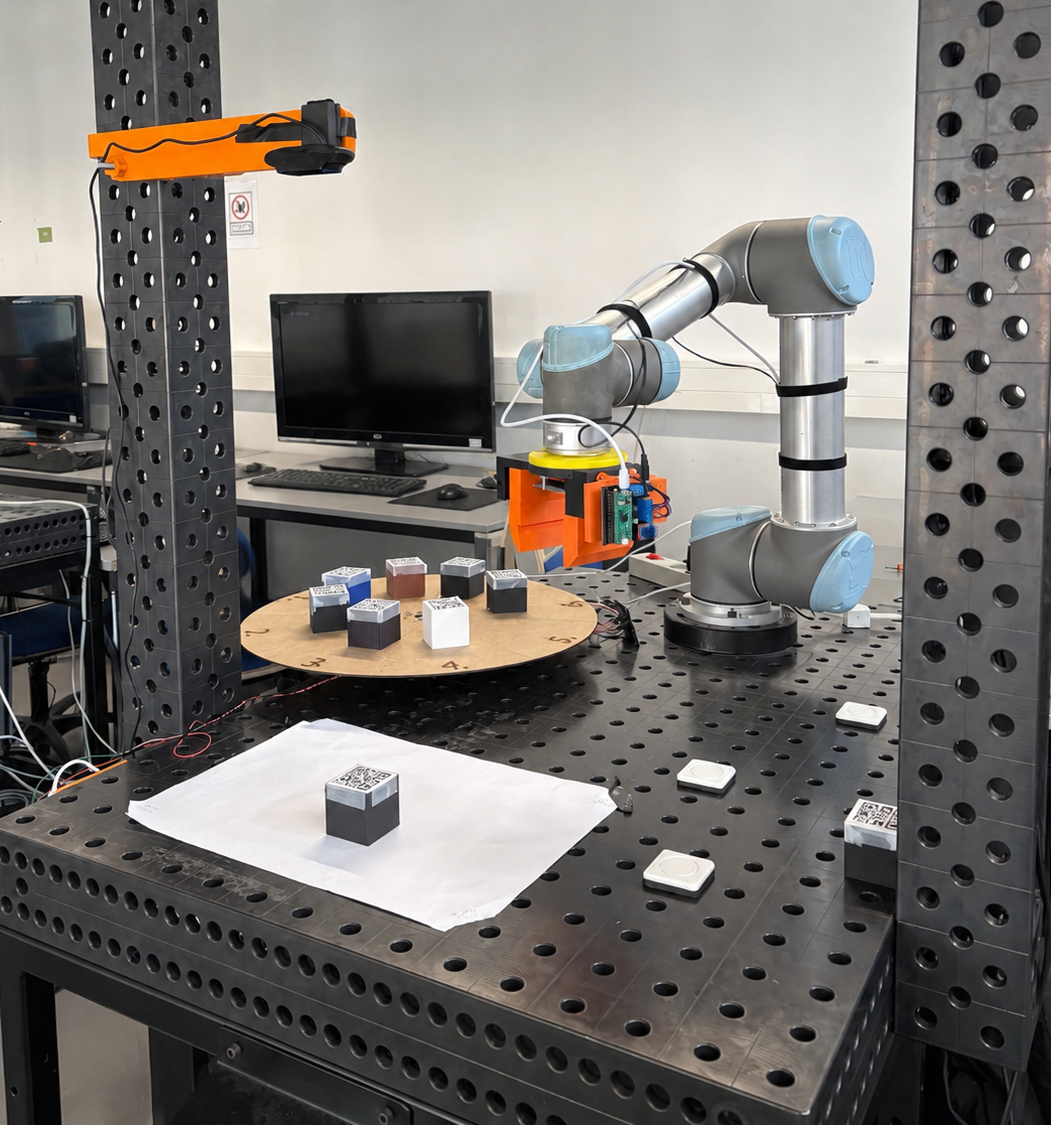
\includegraphics[width=0.9\textwidth]{Appendix/Images/TestSetup.png}
    \caption{Physical test setup of the complete machine.}
    \label{fig:appendix-test-setup}
\end{figure}

\subsection{Web Interface}
\label{app:web-interface}

\begin{figure}[H]
    \centering
    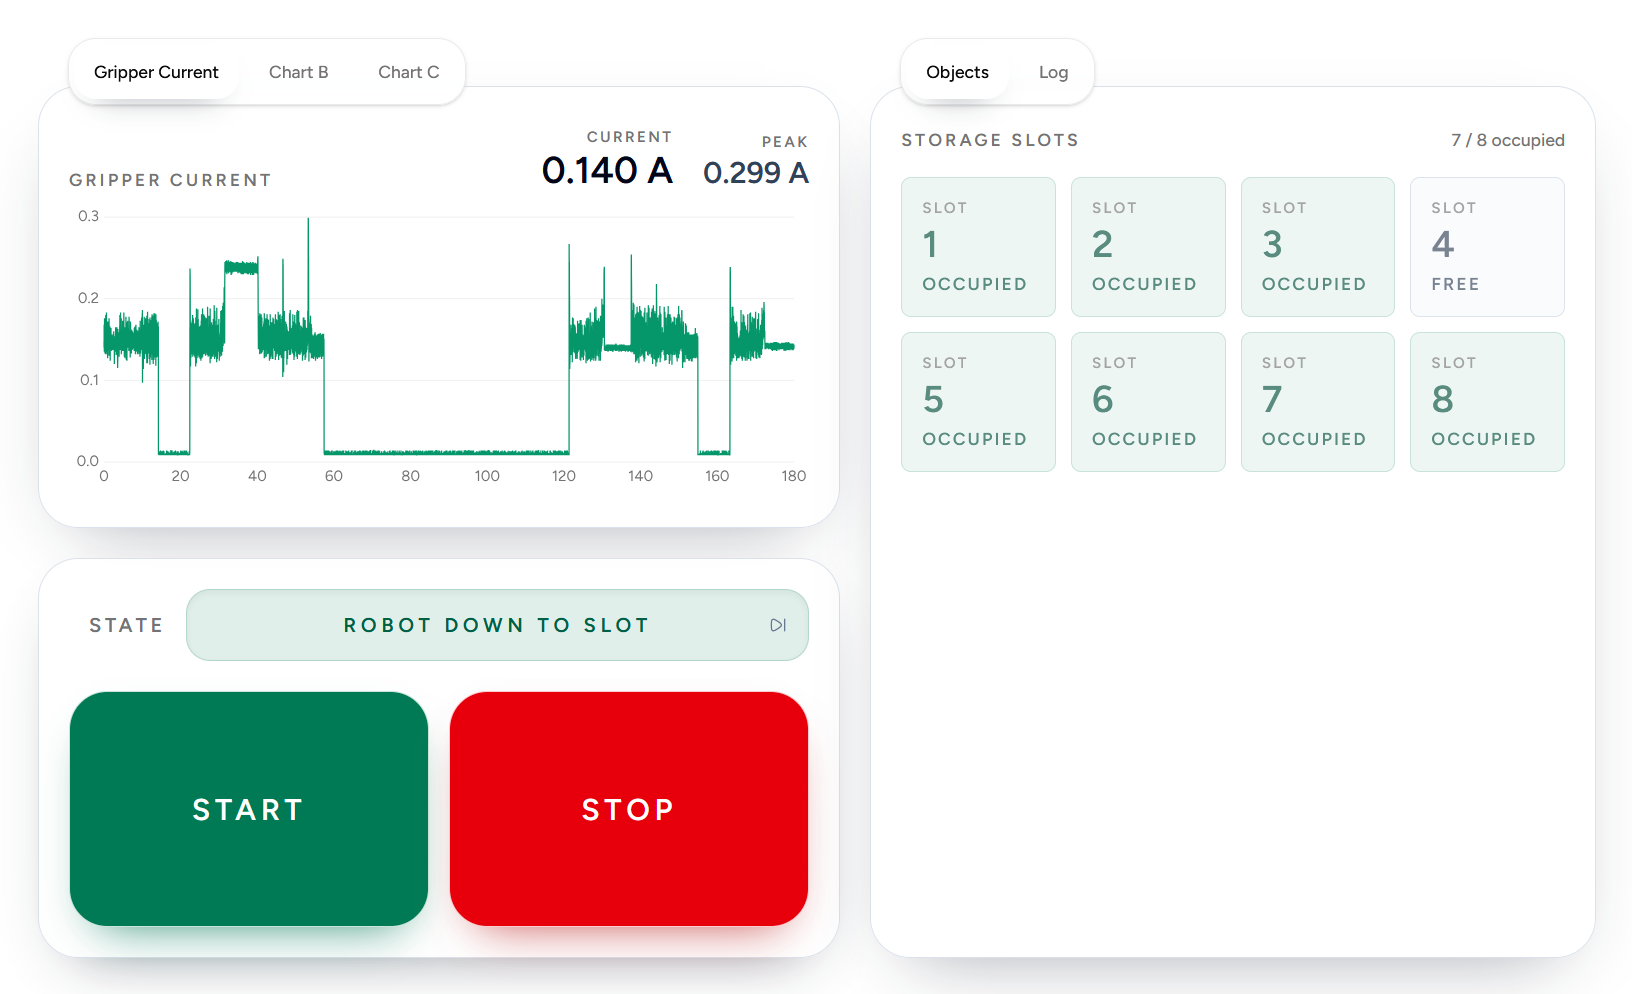
\includegraphics[width=1\textwidth]{Appendix/Images/WebInterface.png}
    \caption{Web interface used for interacting with the system. The top-left panel shows a chart of the gripper current, the bottom-left panel contains the machine controls such as start and stop, and the right side gives an overview of the storage slots with the ability to select a specific slot.}
    \label{fig:appendix-web-interface}
\end{figure}

\subsection{Vision test}
\label{app:Vision-test}
\begin{table}[H]
\centering
\begin{tabular}{|c|c|c|}
\hline
Distance from camera to table & Detailed & Simple \\
\hline
50 cm & 100,0\% & 100,0\% \\
\hline
55 cm & 100,0\% & 100,0\% \\
\hline
60 cm & 99,9\% & 100,0\% \\
\hline
65 cm & 99,8\% & 99,9\% \\
\hline
70 cm & 94,4\% & 100,0\% \\
\hline
\end{tabular}
\caption{Vision ability to find QR codes at different distances}
\label{tab:appendix-vision-findability}
\end{table}


\subsection{Charuco Board}
\label{app:charuco-board}

\begin{figure}[H]
    \centering
    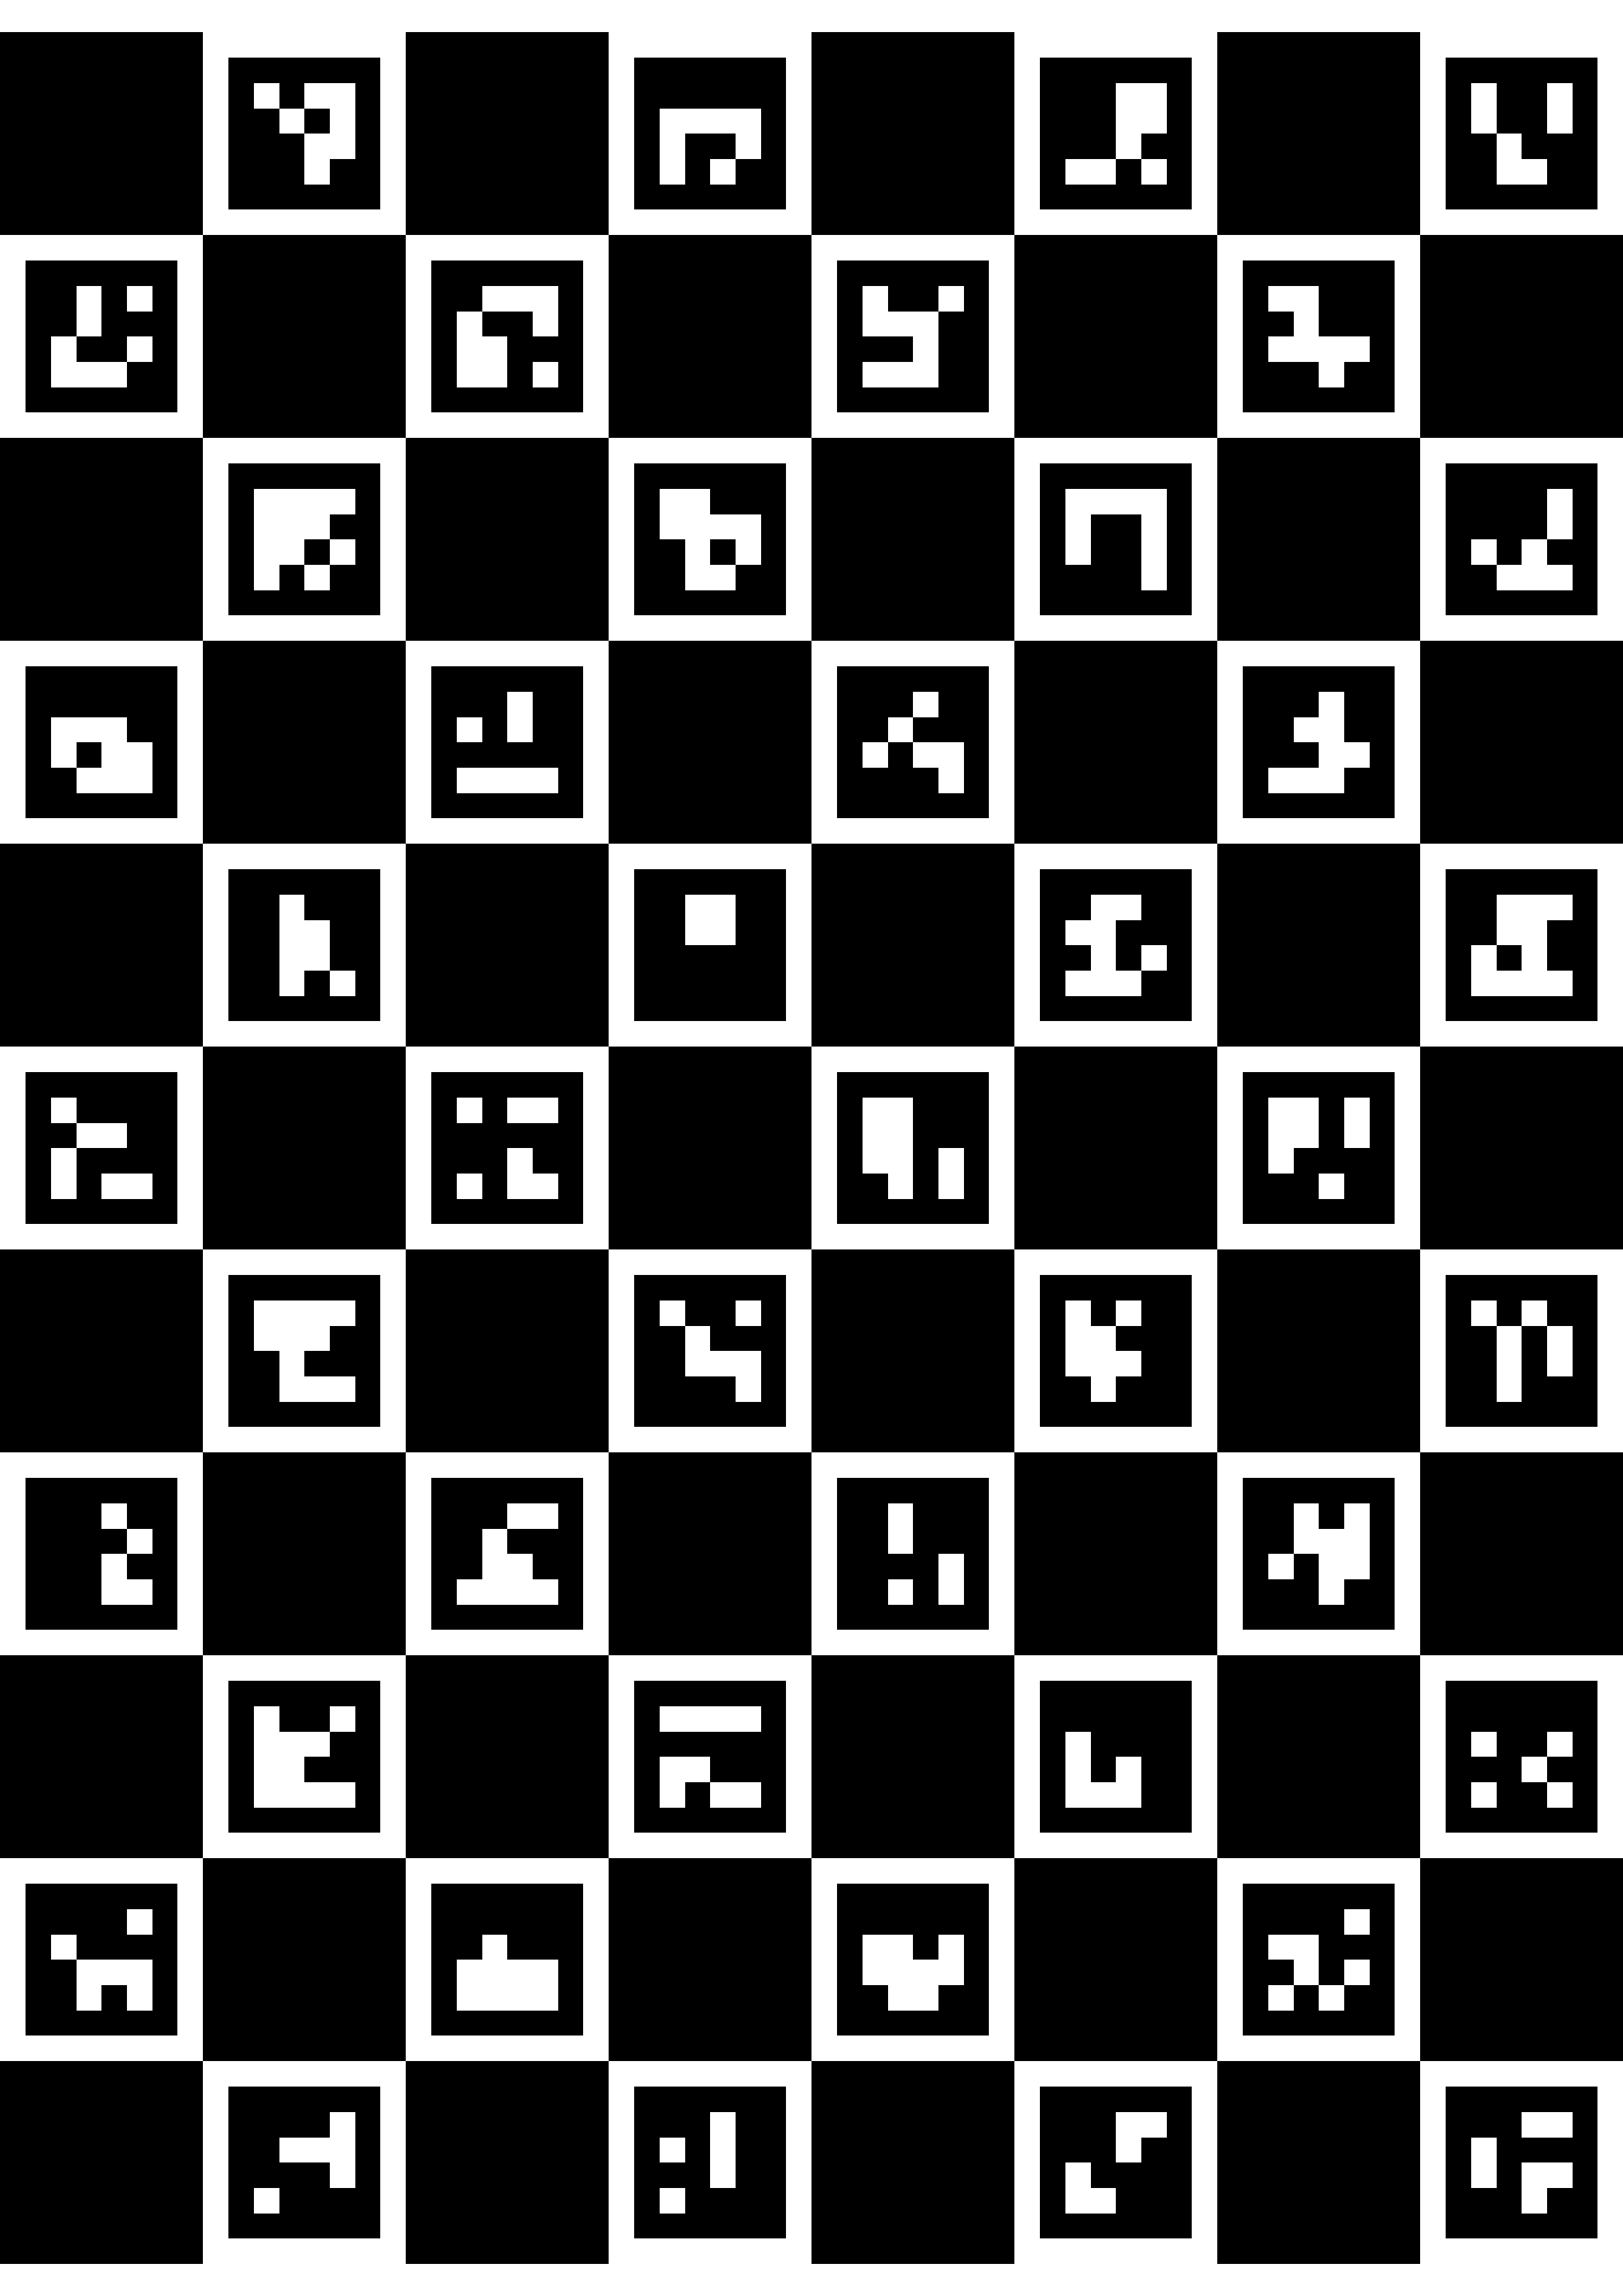
\includegraphics[width=\textwidth]{figures/charuco_board_8x11.png}
    \caption{Charuco board for calibration}
    \label{fig:Charuco_board}
\end{figure}

\subsection{Gripper PCB}
\label{app:gripper-pcb}

\begin{figure}[H]
    \centering
    \begin{subfigure}[t]{0.48\textwidth}
        \centering
        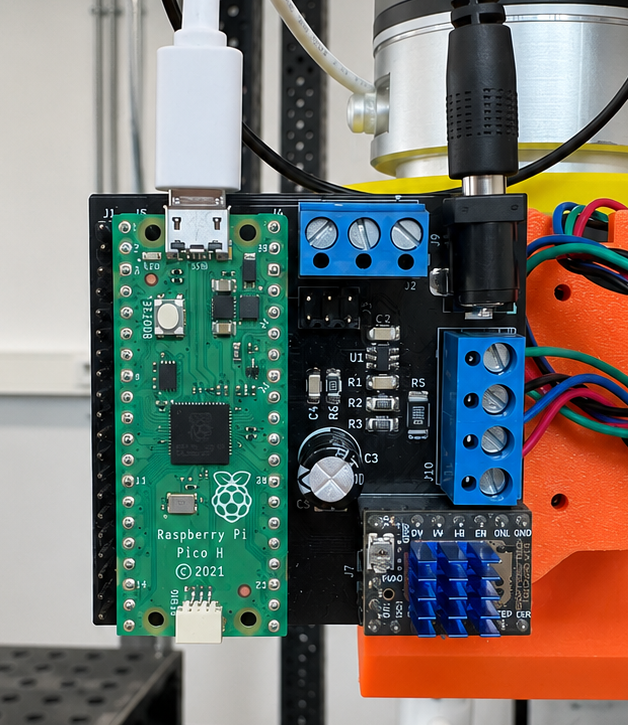
\includegraphics[width=\textwidth]{Appendix/Images/GripperPCB.png}
        \caption{Gripper PCB.}
        \label{fig:gripper-pcb-layout}
    \end{subfigure}
    \hfill
    \begin{subfigure}[t]{0.48\textwidth}
        \centering
        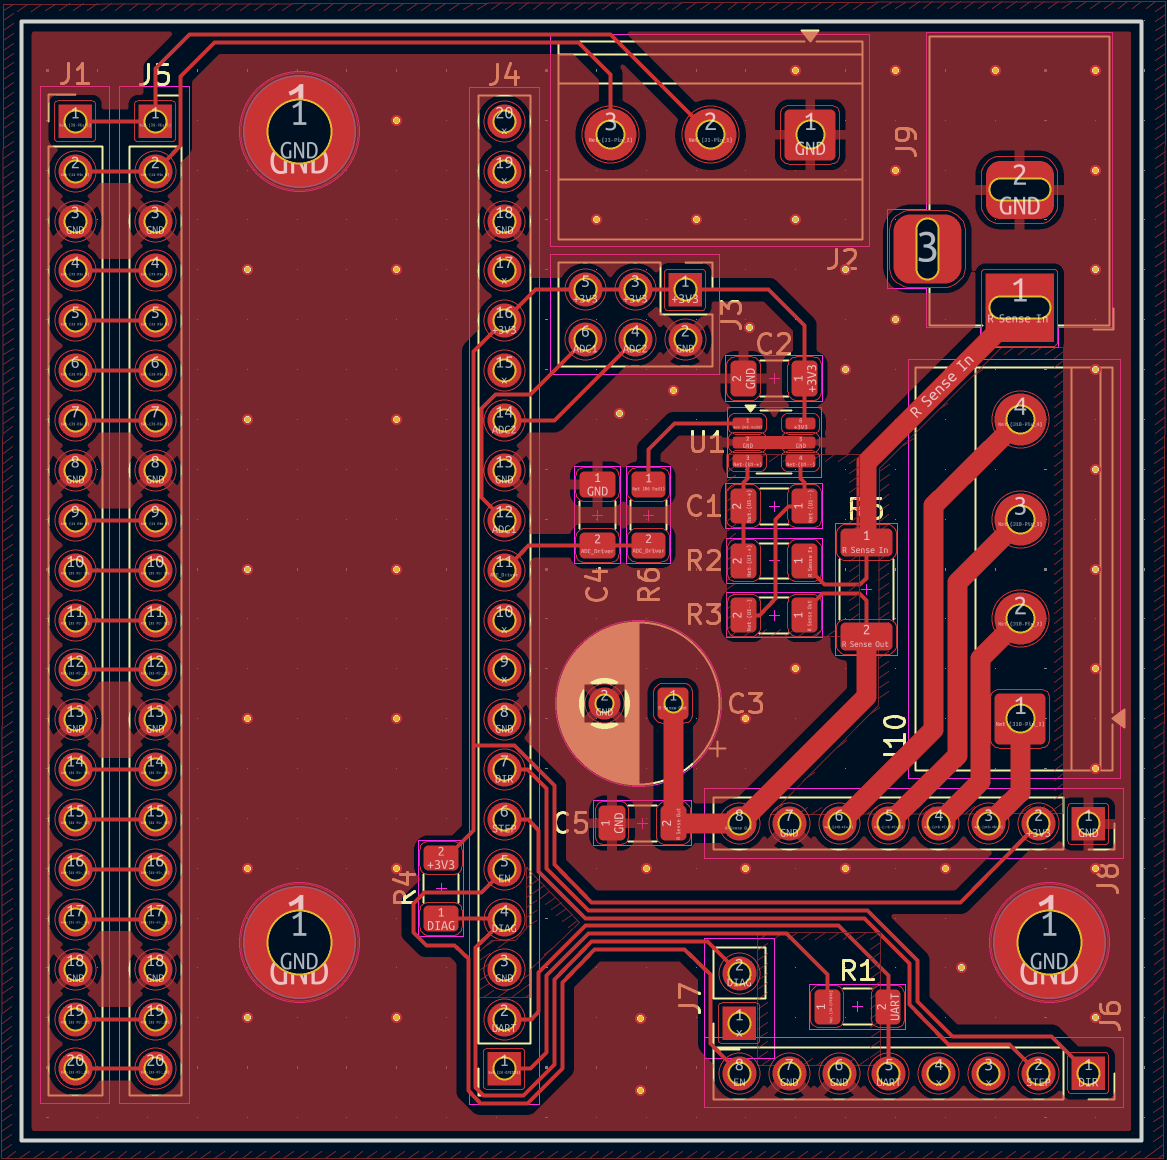
\includegraphics[width=\textwidth]{Appendix/Images/GripperPCBSchematic.png}
        \caption{Gripper PCB layout.}
        \label{fig:gripper-pcb-schematic}
    \end{subfigure}
    \caption{Gripper PCB layout and schematic.}
    \label{fig:gripper-pcb}
\end{figure}

\begin{figure}[H]
    \centering
    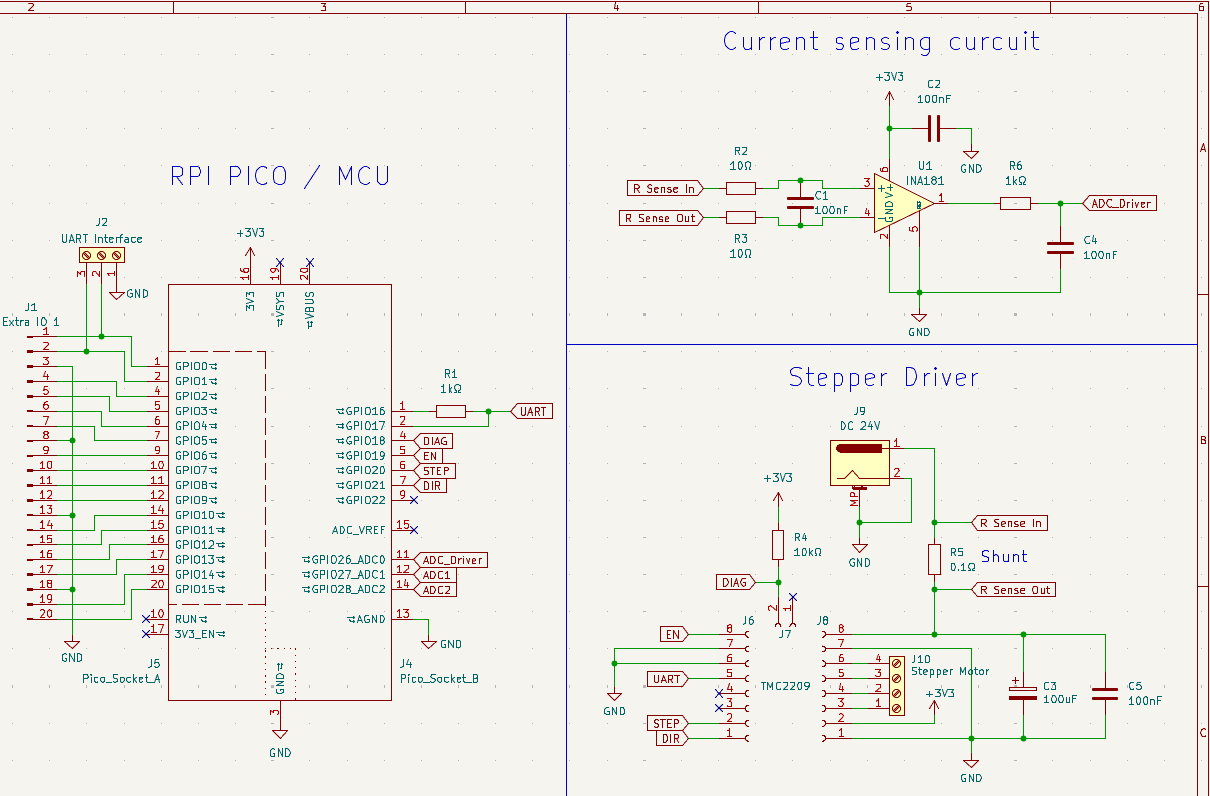
\includegraphics[width=\textwidth]{Appendix/Images/GripperPCBSchematic_real.png}
    \caption{Detailed gripper PCB schematic.}
    \label{fig:gripper-pcb-schematic-detailed}
\end{figure}


\subsection{Ciffer Table for Storage System}
\label{app:ciffertabel}

\begin{figure}[H]
    \centering
    \IfFileExists{figures/CifferTableCarbon02.png}{%
        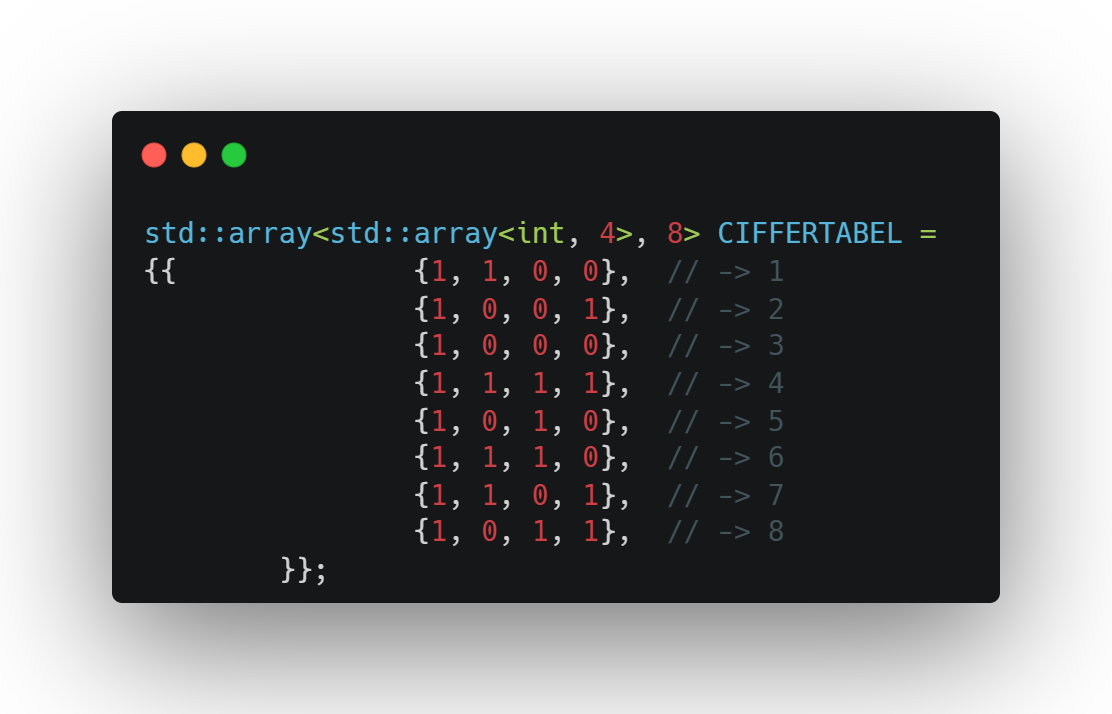
\includegraphics[width=\textwidth]{figures/CifferTablecarbon.png}%
    }{%
        \fbox{\parbox{0.9\textwidth}{\centering Missing image: \texttt{figures/CifferTableCarbon02.png}}}%
    }
    \caption{Ciffer table for the storage system.}
    \label{fig:ciffer-table}
\end{figure}


\section{Digital Appendix}

%Digitale filer/videoer


\subsection{Video Montage}
Recommended to watch on a bigger sized screen:

\url{https://youtu.be/mFUUK1O942Y}


\subsection{Raw video clips}
\label{videos}
%Angle front - occupy slot:
Input-to-Storage cycle:
\url{https://youtube.com/shorts/VWNK5rI8qNM?feature=share} 

%Angle front - free slots:
Storage-to-Output cycle:
\url{https://youtube.com/shorts/XZM1S5uELC4?feature=share} 

%Angle side - occupy + free slots:
%\url{https://youtu.be/dca0lESVhiIshar} 

%Angle Gripper - occupy + free slots:
%\url{https://youtu.be/DyexqrI2SlE} 

%Angle Base - occupy + free slots:
%\url{https://youtu.be/B5A8Hgl0fhc} 

%Web interface - occupy slots:
%\url{https://youtu.be/RSOOtqHnhEQ}

%Web interface - free slots:
%\url{https://youtu.be/wZqRQ5LcIEk} 


Movement test: \url{https://youtube.com/shorts/uH6EiSdd-Ig}

Whole system test: \url{https://www.youtube.com/shorts/CYDVCI7MAuw}


\subsection{Code}

\url{https://github.com/Bosssebastian/2.-semesterprojekt}